% Netzwerkanltung für die Studentenstadt Freimann
% Tex initially created by Maximilian Engelhardt <maximilian.engelhardt@stusta.mhn.de>

%\documentclass[a4paper,12pt,draft]{scrartcl}
\documentclass[a4paper,12pt]{scrartcl}

\usepackage[utf8]{inputenc}
\usepackage{eurosym}
\usepackage{tabularx}
\usepackage[pdftex,final]{graphicx}
\usepackage{wrapfig}
\usepackage[top=1.5cm,bottom=2.5cm,left=1.5cm,right=1.5cm]{geometry}
%\usepackage[margin=2cm]{geometry}
\usepackage{hyperref}


\title{Student residence Studentenstadt Freimann:\\
       Internet configuration guide}
\date{\today}

\begin{document}

\maketitle

\begin{figure}[t!]
   \centering
   \vspace{-20pt}
   
\includegraphics[width=0.8\textwidth,keepaspectratio]{Bilder/StuStaNet_Logo}
   \vspace{-20pt}
\end{figure}

\section*{General information about your Internet connection}

This set-up guide will help you to configure your computer to access the Studentenstadt network as well as the Internet. Before attempting to connect to the Internet please read the terms of use which can be found at the end of your housing contract.

To access the Internet, you require a computer with an ethernet connector (most computers have this feature built-in). Additionally you will need a network cable (RJ-45 patch cable) to connect your computer to the network box located on the wall of your room. Should you not have a network cable, you can purchase a cable from the StuStaNet. See further down for more information

You are responsible for your computer's network activity. You must ensure that it does not pose a threat to any other computer on the network and that it is secured and protected from possible virus- and malware infection. Please note the following points:
\begin{itemize}
    \item Keep your computer updated with the latest security updates
    \item Update your Anti-Virus program regularly
    \item Use a personal firewall
\end{itemize}
If the StuSta detects that your computer is infected by a virus and poses a threat to the computer network, your Internet connectivity will be cut off.

\begin{em}
If your computer shows these symptoms repeatedly, your Internet connectivity will be permanently terminated.
\end{em}

These drastic measures need to be taken, as the entire network can be crippled by one infected computer. Furthermore, the Leibnitz-Rechenzentrum, that provides the Studentenstadt with Internet access, will block all Internet traffic from the entire Studentenstadt, if a computer virus is detected.

\emph{Please note:} The StuStaNet recommends that if you are a beginner and you don't have the know-how of keeping a Windows system secure, you should consider installing a linux operating system such as Ubuntu Linux. Download Ubuntu from \url{http://www.ubuntu.com}.


\section*{Membership in the StuStaNet~e.V.}

The membership in the StuStaNet~e.V. is a once-off fee of \EUR{10} and has a number of advantages such as in addition to the Proxy-Internet, the "Real Internet" over a masquerader, an e-mail address, webspace with PHP and database support\footnote{\url{https://wiki.stusta.mhn.de/Liste\_der\_Vereinsdienste}}.

You can join the StuStaNet~e.V. in one of our consultation hours, which are Mondays and Thursdays from 19.00 to 19.30 in the blue house, room 0028, during the semester.

If you are interested in our network and our servers or if you would like to contribute some ideas, you can become a house administrator (elections are at the beginning of each semester in the different houses) or just come past our monthly meeting (Adminrat). This meeting takes place on the first Thursday of every month at 20.00 in the Teestube\footnote{The Teestube is located in the 20th floor of the Hanns Seidel Hauses (HSH), Christoph-Probst-Str. 16}.

\section*{More Information}

For problems please consult the Stusta-Wiki and the Infoseite:

\begin{center}
  \begin{tabularx}{\linewidth}{|lX|}
    \hline
    \url{http://wiki.stusta.mhn.de/} & Network help, information about living in the Studentenstadt, Shopping in the area, Doctors, Nightlife..\\
    \hline
    \url{http://info.stusta.mhn.de/} & Announcements and general information about the StuSta\\
    \hline
  \end{tabularx}
\end{center}
Should you experience problems configuring your Internet access, you can contact a house administrator. A list of house administrators is located on the ground floor of your house.

Keep in mind that the administrators are only responsible for network-related problems.

\newpage
\section*{Tips on securing your computer}

Here are a few tips on securing your computer against harmfull software.

\subsection*{Anti virus programs}
\paragraph*{Windows}
\begin{center}
  \begin{tabularx}{\linewidth}{|p{.2\linewidth}XX|}
    \hline
    Name & Website & Description\\
    \hline \hline
    Avira AntiVir & \url{http://www.free-av.com/} & free, since 1988\\
    \hline
    Microsoft Security Essentials & \url{http://www.microsoft.com/security\_essentials/} & free, by Microsoft, also anti spyware\\
    \hline
    Sophos Antivirus & \url{http://sophos.lrz-muenchen.de/} & Commercial software which is supplied by the LRZ, that can be used for free by students\\
    \hline
    avast! & \url{http://www.avast.de/} & Home Edition free for private use\\
    \hline
  \end{tabularx}
\end{center}

There are numerous more anti virus programs which however are commercial and require a license such as Kaspersky, Norton and McAffee.

\paragraph*{Linux and MacOS X (Apple)}

There is no need to use an anti virus package with either of these operating systems. Due to the small market capitalization and different software architecture, these platforms are virus-free (for now).
\subsection*{Antispywareprogramme}

Spyware is used to spy on users and to collect personal information. You can find more information on Wikipedia\footnote{\url{http://en.wikipedia.org/wiki/Spyware}}.

\begin{center}
  \begin{tabularx}{\linewidth}{|p{.18\linewidth}Xp{.3\linewidth}|}
    \hline
    Name & Website & Description\\
    \hline \hline
    Windows Defender & \url{http://www.microsoft.com/germany/windows/products/winfamily/defender/default.mspx} & Integrated in Microsoft Security Essentials\\
    \hline
    Spybot, Search \& Destroy & \url{http://www.safer-networking.org/} & Free for private use\\
    \hline
    Ad-Aware & \url{http://www.lavasoft.com/products/select\_your\_product.php} & Free version available\\
    \hline
  \end{tabularx}
\end{center}

There are numerous more anti spyware programs, most of which are commercial software. These usually come in combination with a firewall or anti virus program.

\subsection*{Personal Firewalls}

A firewall controls the connection between a computer and the network to which the computer is connected to. You can find more information on Wikipedia\footnote{\url{http://en.wikipedia.org/wiki/Personal\_Firewall}}.

Almost every anti virus program has an integrated firewall and even anti spyware software.

In general, the integrated firewall of an operating system is not enough to ensure complete protection.
\newpage

\section*{Network configuration}

Each network point is assigned 8 IP addresses and the IP range is marked on the outlets. If this isn't the case or if the sticker is unreadable, please fill in a repair form which can be found in the entrance hall of the house management building.

\subsection*{Overview}

To successfully connect to the Internet you need to ensure the following:
\begin{itemize}
    \item The connection to the network point
    \item Configuration of the network settings in your operating system
    \item Entry of proxy information~/ proxy script into your Internet browser
\end{itemize}


\begin{center}
  \begin{tabularx}{\linewidth}{|lXp{.2\linewidth}|}
    \hline
    Setting & Value & Example \\
    \hline \hline
    IP address & \nolinkurl{10.150.xxx.yyy} - \nolinkurl{10.150.xxx.zzz}, \newline 8 addresses are available which are marked on the network point & \nolinkurl{10.150.243.16} - \nolinkurl{10.150.243.23} \\
    \hline
    Subnet mask & \nolinkurl{255.255.255.0} & \\
    \hline
    Standard gateway & \nolinkurl{10.150.xxx.254} \newline first three blocks like the IP address, fourth block \nolinkurl{254} & \nolinkurl{10.150.243.254} \\
    \hline
    DNS server (Nameserver) & \nolinkurl{10.150.127.2} \newline \nolinkurl{10.150.125.2} & \\
    \hline
    DNS suffix (Domainname) & \nolinkurl{stusta.mhn.de} & \\
    \hline
    Proxy script & \multicolumn{2}{l|}{\nolinkurl{http://wpad.stusta.mhn.de/proxy.pac}} \\
    \hline
    Proxy server (manual) & \multicolumn{2}{l|}{\nolinkurl{http://proxy.stusta.mhn.de:3128}} \\
    \hline
  \end{tabularx}
\end{center}

You must either use the proxy script or the manual proxy configuration although the use of the \emph{proxy script} is the preferred method.

\subsection*{Connection to the network point}

Only use the left network connection point!

Beware! It is \emph{prohibited} to connect a telephone, ISDN equipment or any similar devices to the left network connection point as these cause massive network outages in the Sudentenstadt and can cause damage to network hardware.

\subsection*{E-mail, Skype, ICQ, Online games, ...}

The Internet connection in the Sudentenstadt is intended for educational purposes only.

The standard Internet access in the Studentenstadt is limited to browsing only (Connections via the HTTP proxy) as well as internal connections to the Munich Scientific Network. Sending e-mail over POP3~/ IMAP, using instant messaging and playing online games only works with a StuStaNet~e.V. membership (see above).


\newpage

\begin{figure}[t!]
    \raggedleft
    \vspace{-20pt}
    
\includegraphics[height=1cm,keepaspectratio]{Bilder/Ubuntu_logo}
    \vspace{-20pt}
\end{figure}

\section*{Step by step instructions}
\subsection*{Ubuntu settings}
\begin{enumerate}
    \item Open the network configuration dialog by clicking on System $\rightarrow$ Settings $\rightarrow$ Network Settings.
    \item Select your network card in the first tab (normally eth0) and click on edit.
    \item Click on the IPv4-Settings tab and change the method to Manually.
    \item Under addresses click on Add.
      \begin{figure}[h!]
        \centering
        \begin{minipage}[c]{0.45\linewidth}
          \centering
          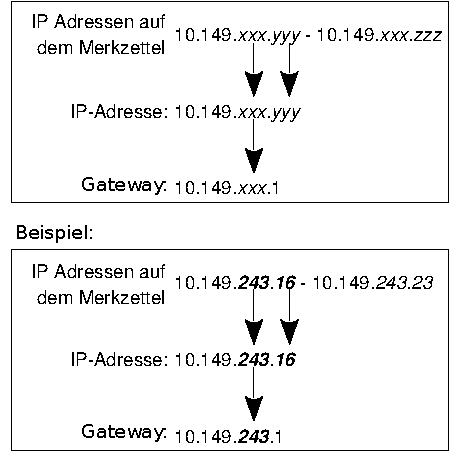
\includegraphics[width=\linewidth,keepaspectratio]{Bilder/IP_Gerneric}
        \end{minipage}
        \begin{minipage}[c]{0.5\linewidth}
          \centering
          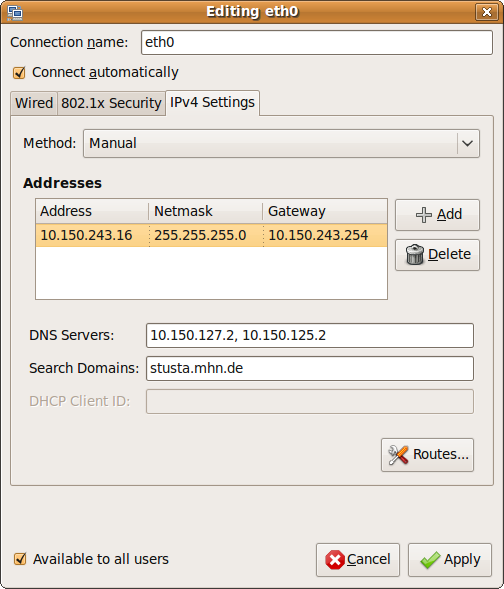
\includegraphics[width=\linewidth,keepaspectratio]{Bilder/IP_Ubuntu_EN}
          \caption{Example network configuration in Ubuntu Linux}
          \vspace{-10pt}
        \end{minipage}
      \end{figure}
    \item Now type in the IP address, the subnet mask, the gateway, the DNS and the search domain. The DNS server addresses are \nolinkurl{10.150.127.2} and \nolinkurl{10.150.125.2}, the search domain is \nolinkurl{stusta.mhn.de} and the subnet mask is \nolinkurl{255.255.255.0}. You can find your IP address on the sticker on the network point. Confirm the settings with OK and close the window.
\end{enumerate}

\paragraph*{Global proxy settings}
You can define a global proxy server in Ubuntu so that you don't have to configure it for each browser individually.
\begin{enumerate}
    \item Open the network proxy settings by clicking on System $\rightarrow$ Settings $\rightarrow$ Network Proxy.
    \item At the bottom of the window, mark the automatic proxy configuration box and enter this auto configuration URL: \url{http://wpad.stusta.mhn.de/proxy.pac}\ . Close the window.
\end{enumerate}
$\rightarrow$ Your Internet access is now configured.



\newpage
\enlargethispage{20pt}

\begin{figure}[t!]
    \raggedleft
    \vspace{-20pt}
    
\includegraphics[height=1cm,keepaspectratio]{Bilder/Windows_logo}
    \vspace{-20pt}
\end{figure}

\section*{Step by step instructions}
\subsection*{Windows settings}
\begin{enumerate}
    \item Open Control Panel by clicking on Start $\rightarrow$ Control Panel.
\end{enumerate}
\vspace{-15pt}
\paragraph*{Windows XP}
\begin{enumerate}
     \setcounter{enumi}{1}
     \item Click on Network and Internet Connections.
     \item Click on Network Connections.
     \item Right click on the Local Area Connection and select properties.
\end{enumerate}
$\rightarrow$ Continue at point 5.
\vspace{-10pt}
\paragraph*{Windows Vista}
\begin{enumerate}
    \setcounter{enumi}{1}
    \item Click on "Network and Internet" then on "View network status and tasks".
    \item Click on "Change adapter settings" and then right click on the Local Area Connection and select properties.
    \setcounter{enumi}{4}
    \item Select Internet Protocol Verson 4 (TCP/IPv4) (Windows Vista)/ Internet Protocol  (TCP/IP) (Windows XP) and click on Properties.
    \item Now type in the IP address, the subnet mask, the Default gateway and the DNS Server. The DNS Server addresses are \nolinkurl{10.150.127.2} and \nolinkurl{10.150.125.2}, the Subnet mask is \nolinkurl{255.255.255.0}. You can find your IP address on the sticker on the network point.
      \begin{figure}[h!]
	\centering
        \vspace{-5pt}
        \begin{minipage}[c]{0.45\linewidth}
          \centering
          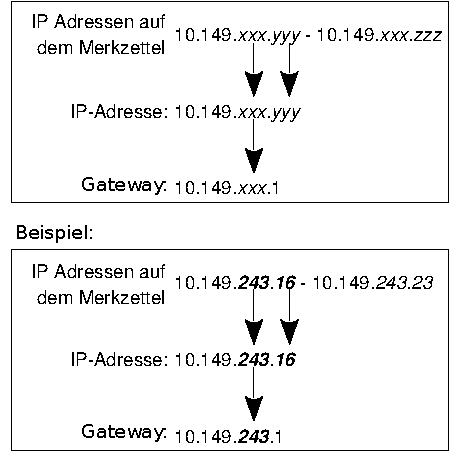
\includegraphics[width=\linewidth,keepaspectratio]{Bilder/IP_Gerneric}
        \end{minipage}
        \begin{minipage}[c]{0.48\linewidth}
          \centering
          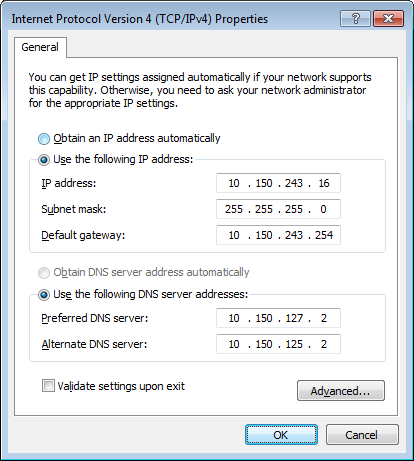
\includegraphics[width=\linewidth,keepaspectratio]{Bilder/IP_Windows_EN}
          \caption{Example network configuration in Windows Vista}
        \end{minipage}
      \vspace{-15pt}
      \end{figure}
    \item Click on Advanced and click on the DNS tab. Klicken Sie auf Erweitert und wählen im folgenden Dialog den Reiter DNS aus. Type \nolinkurl{stusta.mhn.de} in the DNS suffix for this connection field.
    \item Confirm the settings with OK and close the window.
\end{enumerate}
$\rightarrow$ Continue with the browser settings.



\newpage

\begin{figure}[t!]
    \raggedleft
    \vspace{-20pt}
    
\includegraphics[height=1cm,keepaspectratio]{Bilder/OSXLeopard}
    \vspace{-20pt}
\end{figure}

\section*{Step by step instructions}
\subsection*{Mac OS X settings}
\begin{enumerate}
    \item Click on the Apple logo (top left) and select System Preferences $\rightarrow$ Network.
    \item Select the Ethernet connection.
    \item Set the Configure IPv4 drop-down box to Manually.
    \item Now type in the IP address, the subnet mask, the gateway, the DNS and the search domain. The DNS server addresses are \nolinkurl{10.150.127.2} and \nolinkurl{10.150.125.2}, the search domain is \nolinkurl{stusta.mhn.de} and the subnet mask is \nolinkurl{255.255.255.0}. You can find your IP address on the sticker on the network point. Confirm the settings with Apply.
      \begin{figure}[h!]
      \centering
%      \vspace{-5pt}
        \begin{minipage}[c]{0.38\linewidth}
          \centering
          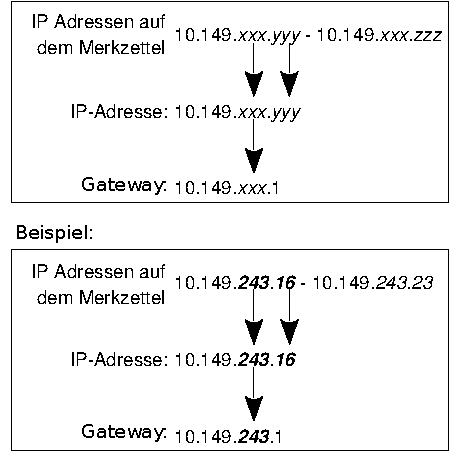
\includegraphics[width=\linewidth,keepaspectratio]{Bilder/IP_Gerneric}
        \end{minipage}
        \begin{minipage}[c]{0.60\linewidth}
          \centering
          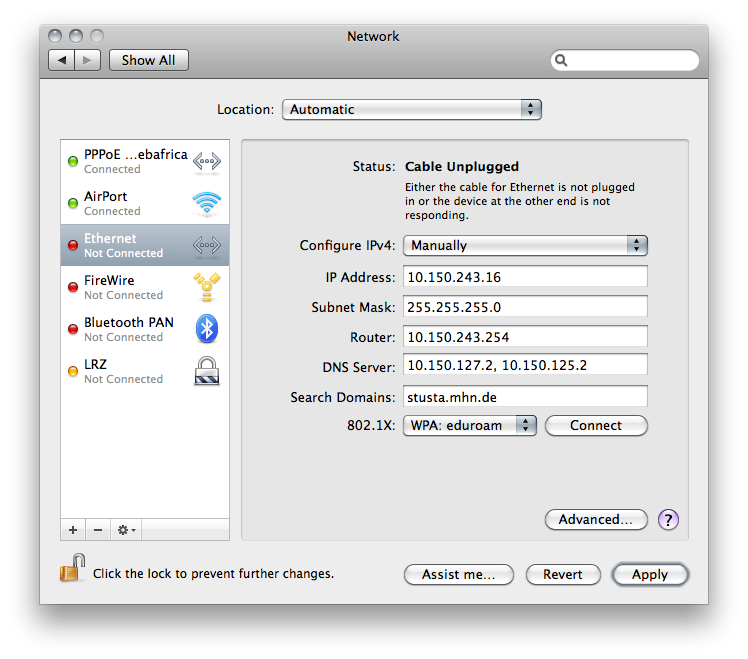
\includegraphics[width=\linewidth,keepaspectratio]{Bilder/IP_Mac_EN}
          \caption{Example network configuration in Mac OS X}
        \end{minipage}
%      \vspace{-15pt}
      \end{figure}
\end{enumerate}

\paragraph*{Global proxy settings}
You can define a global proxy server in Mac OS X so that you don't have to configure it for each browser individually, however Firefox still needs an individual configuration (see Browser settings)
%\begin{wrapfigure}{r}{0.4\textwidth}
%  \vspace{-20pt}
%  \begin{center}
%    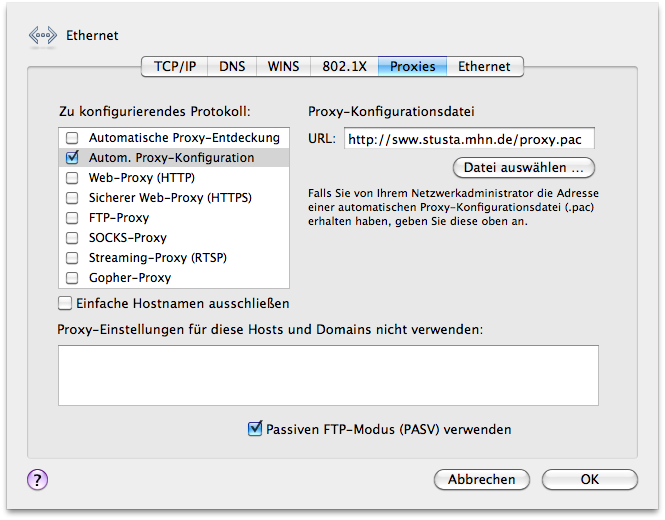
\includegraphics[width=0.48\textwidth,keepaspectratio]{Bilder/Proxy_MAC}
%  \end{center}
%  \vspace{-20pt}
%  \caption{Beispielhafte Proxyeinstellungen unter Mac OS~X}
%  \vspace{-10pt}
%\end{wrapfigure}
\begin{enumerate}
    \item Click on Advanced and select the Proxies tab
    \item Mark the checkbox next to Automatic Proxy Configuration and type in this URL \url{http://wpad.stusta.mhn.de/proxy.pac}\ . Click on OK and select Apply one more time. You can now close System Preferences.
\end{enumerate}
$\rightarrow$ Your Internet access is now configured.

\newpage

\section*{Browsereinstellungen}

\begin{wrapfigure}{r}{0.5\textwidth}
%  \vspace{-20pt}
  \begin{center}
    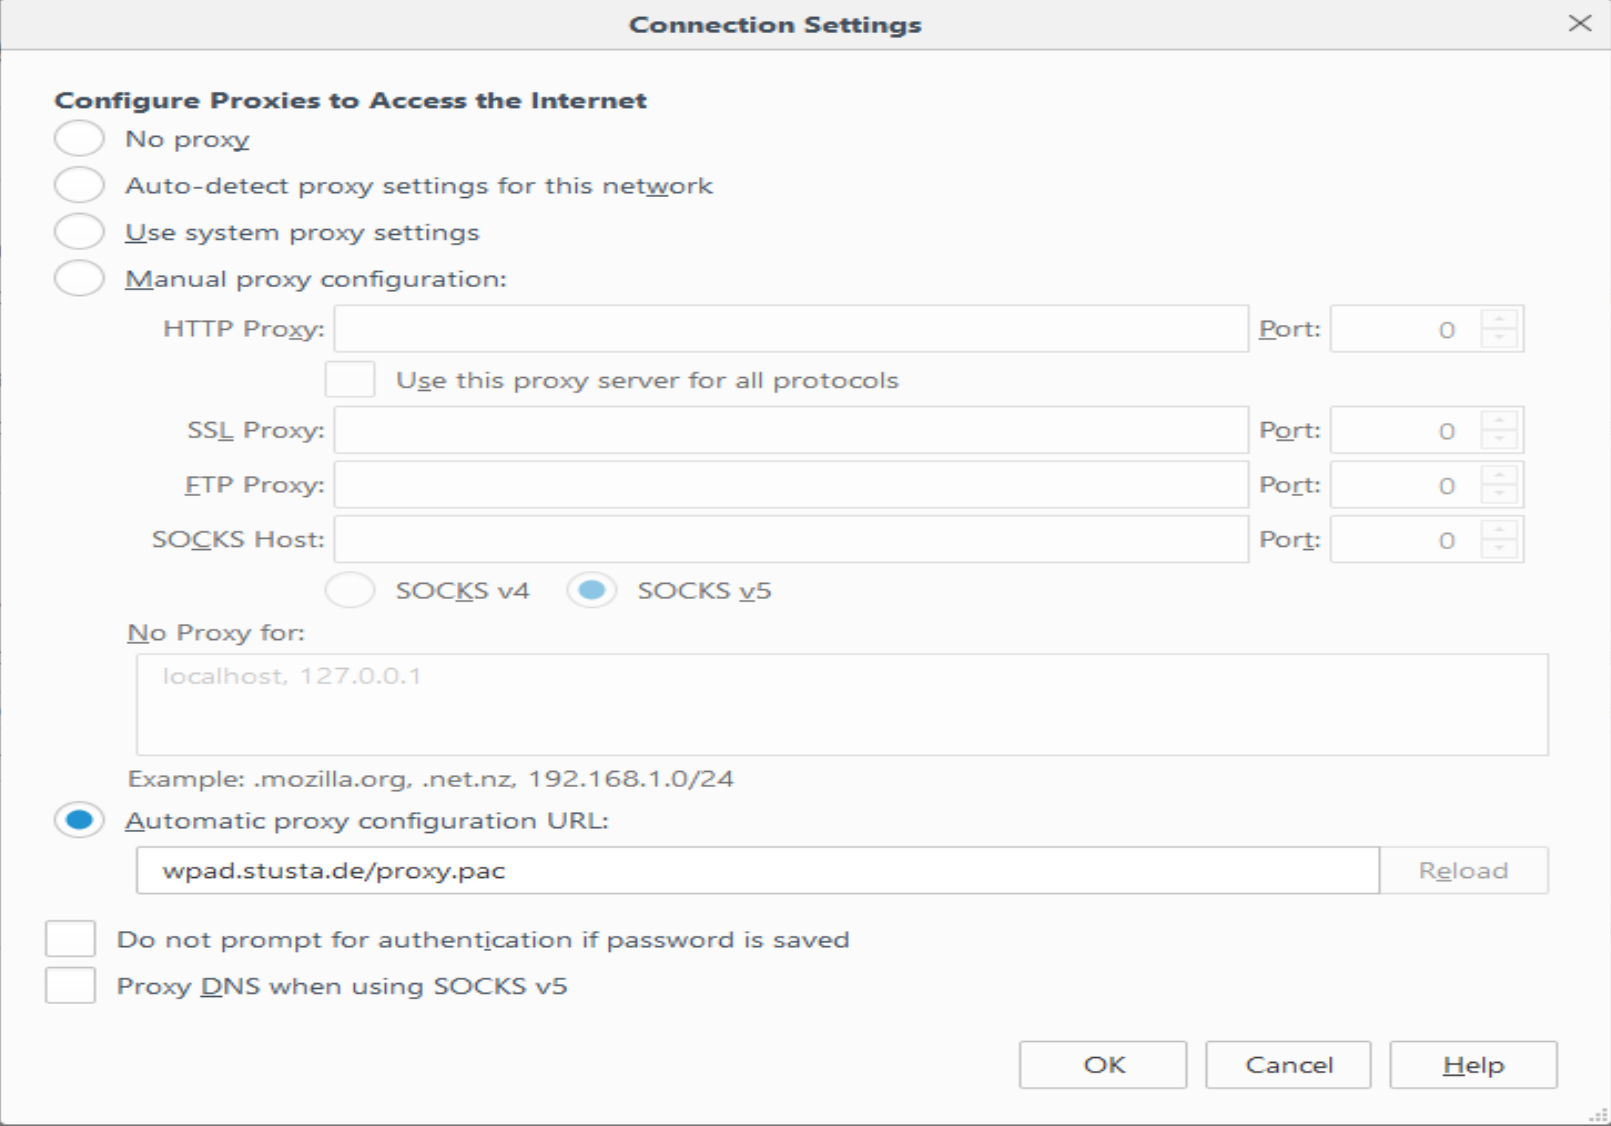
\includegraphics[width=0.5\textwidth,keepaspectratio]{Bilder/Proxy_Firefox_EN}
  \end{center}
%  \vspace{-20pt}
  \caption{Configuring the proxy script in Mozilla Firefox}
%  \vspace{-10pt}
\end{wrapfigure}

\subsection*{
\includegraphics[height=1.2cm,keepaspectratio]{Bilder/Firefox_35_logo} Mozilla Firefox}
\begin{enumerate}
    \item Start Firefox.
    \item Click on Edit $\rightarrow$ Preferences.
    \item Click on advanced and select the Network tab.
    \item Click on Settings.
    \item Select the bottom most radio button and use \\ \url{http://wpad.stusta.mhn.de/proxy.pac} as the Automatic proxy configuration URL.
    \item Confirm with OK and close the remaining windows.
\end{enumerate}
$\rightarrow$ Your Internet access is now configured.


\begin{wrapfigure}{r}{0.5\textwidth}
%  \vspace{-20pt}
  \begin{center}
    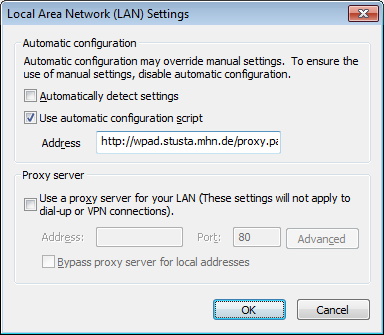
\includegraphics[width=0.5\textwidth,keepaspectratio]{Bilder/Proxy_IE_EN}
  \end{center}
%  \vspace{-20pt}
  \caption{Configuring the proxy script in Internet Explorer}
%  \vspace{-10pt}
\end{wrapfigure}

\subsection*{
\includegraphics[height=1.2cm,keepaspectratio]{Bilder/Internet_Explorer_7_Logo} Internet Explorer}
\begin{enumerate}
    \item Start Internet Explorer.
    \item Click on Tools and select Internet Options.
    \item In the Connections tab, select the LAN Settings button.
    \item Mark the Use automatic configuration script checkbox and type in this URL: \\ \url{http://wpad.stusta.mhn.de/proxy.pac}
    \item Confirm with OK and close the remaining windows.
\end{enumerate}
$\rightarrow$ Your Internet access is now configured.

\newpage
\begin{wrapfigure}{r}{0.5\textwidth}
%  \vspace{-20pt}
  \begin{center}
    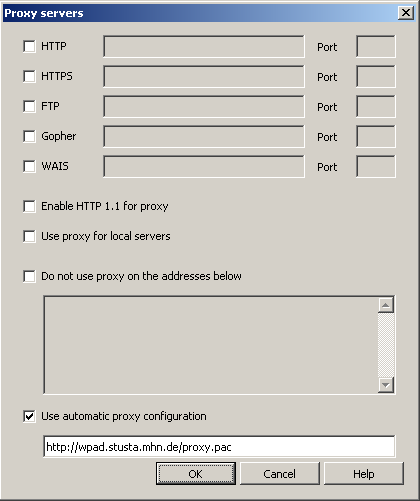
\includegraphics[width=0.5\textwidth,keepaspectratio]{Bilder/Proxy_Opera_EN}
  \end{center}
%  \vspace{-20pt}
  \caption{Configuring the proxy script in Opera}
%  \vspace{-10pt}
\end{wrapfigure}

\subsection*{
\includegraphics[height=1.2cm,keepaspectratio]{Bilder/Opera_O} Opera}
\begin{enumerate}
    \item Start Opera.
    \item Click on Tools and select Settings $\rightarrow$ Preferences.
    \item Click on the Advanced tab, select the Network category on the left and click on the Proxy servers button.
    \item Mark the automatic proxy configuration script checkbox and type in this URL: \\ \url{http://wpad.stusta.mhn.de/proxy.pac}
    \item Close both windows by clicking on OK.
\end{enumerate}
$\rightarrow$ Your Internet access is now configured.


\end{document}

